% $Id: conclusion.tex 
% !TEX root = main.tex

%%
\section{Adaptive \ac{RL} Agents with Changing Behavior}
\label{sec:implementation}

This section introduces \adaptiverl, our proposed approach for enabling \ac{RL} agents to dynamically adapt their behavior in response to evolving environmental conditions. Our method allows agents to pursue varying objectives throughout their operational lifespan and acquire new capabilities as tasks change over time. The implementation is publicly available\footnote{Available at: \url{https://github.com/rulas99/rl_uniandes}}.

The conceptual foundation of \adaptiverl aligns with the idea proposed by~\citet{abel2023definitioncontinualreinforcementlearning}, emphasizing continual adaptation rather than converging to a fixed solution for a problem. We extend tabular Q-learning by integrating adaptive mechanisms, enabling agents to dynamically adjust their learning strategies based on changes detected in their environment. Similar to the approach described by~\citet{norman2024firstexploreexploitmetalearningsolve}, our agent initially explores the environment each time a change is detected, subsequently exploiting the gathered knowledge. This strategy facilitates rapid convergence to new environment configurations without entirely discarding previously acquired knowledge.

To achieve such dynamic behavior adaptation, we propose the following adaptive mechanisms integrated into the agent’s learning parameters: learning rate \& exploration rate integrated with a concept drift detection mechanism.

We implement a dynamic adjustment of the learning rate based on the Temporal Difference (TD) error, defined as follows in \eqref{eq:td_error}.
\begin{equation}
    \label{eq:td_error}
    TD_{error} = r_{t+1} + \gamma \cdot \underset{a}{\max} Q(s_{t+1}, a) - Q(s_t, a_t)
\end{equation}
This error measures the discrepancy between the agent’s predicted reward and the actual reward received. The dynamic learning rate ($\alpha^*$) adapts according to this TD error as shown in \eqref{eq:dynamic_learning_rate}.
\begin{equation}
    \label{eq:dynamic_learning_rate}
    \alpha^* = \alpha + (\alpha_{\max}-\alpha) \cdot \frac{1}{1 + e^{-(|TD_{error}|-k)}}
\end{equation}
In this formulation, $\alpha$ is the base learning rate, and $\alpha_{\max}$ represents its upper bound (e.g., 0.99). The parameter $k$ modulates the sensitivity of the learning rate to the TD error, requiring careful tuning depending on the specific characteristics of the environment and learning context. High TD errors trigger a larger learning rate, promoting faster updates during exploration, while lower TD errors result in more stable, conservative learning during exploitation phases.

\begin{figure*}
    \centering
    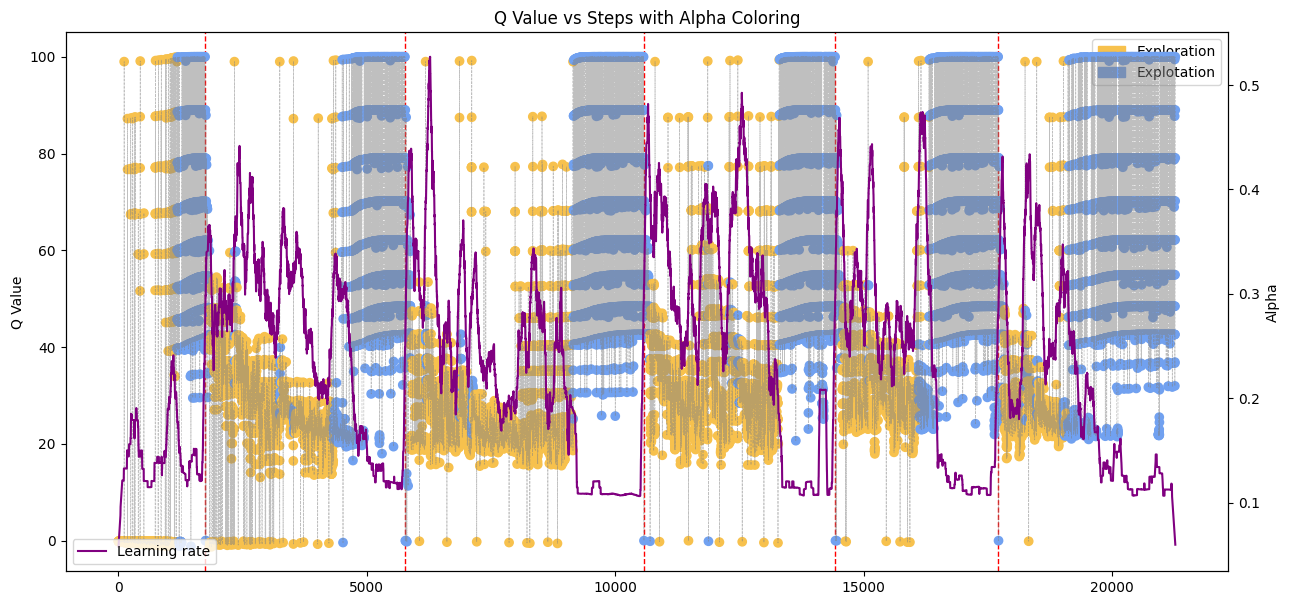
\includegraphics[width=\textwidth]{figures/alpha.png}
    \caption{Figure description}
    \label{fig:alpha}
\end{figure*}

Following the methodologies of~\citet{mignon2017adaptive} and~\citet{networkdynamicrl}, we implement the PH-test to detect significant shifts in the reward distribution at the end of each episode. The PH-test calculates a cumulative difference between observed rewards ($r_j$) and the running mean reward ($\bar{r}$), incorporating a sensitivity parameter ($\delta$). A concept drift (environmental change) is flagged when this cumulative difference surpasses a predefined threshold. Selecting an appropriate threshold value is crucial, as it determines the sensitivity of drift detection. Higher thresholds result in more conservative detection, while lower thresholds increase sensitivity to changes.

Building on the concept drift detection mechanism, and inspired by~\citet{mignon2017adaptive}, we adaptively increase the exploration rate ($\varepsilon$) when a concept drift is detected by PH-test. The goal is to facilitate exploration immediately after environmental changes to acquire new knowledge:
\begin{equation}
    \label{eq:epsilon_greedy}
    \varepsilon^* = \varepsilon_{\min} + (1-\varepsilon_{\min}) e^{-ct}
\end{equation}
Here, $\varepsilon_{\min}$ (e.g., 0.1) is the minimal exploration rate, $c$ controls the rate of decay, and $t$ is the timestep. A higher value of $c$ results in faster decay, enabling the agent to swiftly return to exploitation after sufficient exploration. This adaptive exploration ensures the agent maintains a balance between exploring new environment dynamics and leveraging established knowledge. It is crucial to maintain high levels of exploration after a concept drift is consistency detected, so the agent can learn new policies  without forgetting previously learned ones.

\begin{figure*}
    \centering
    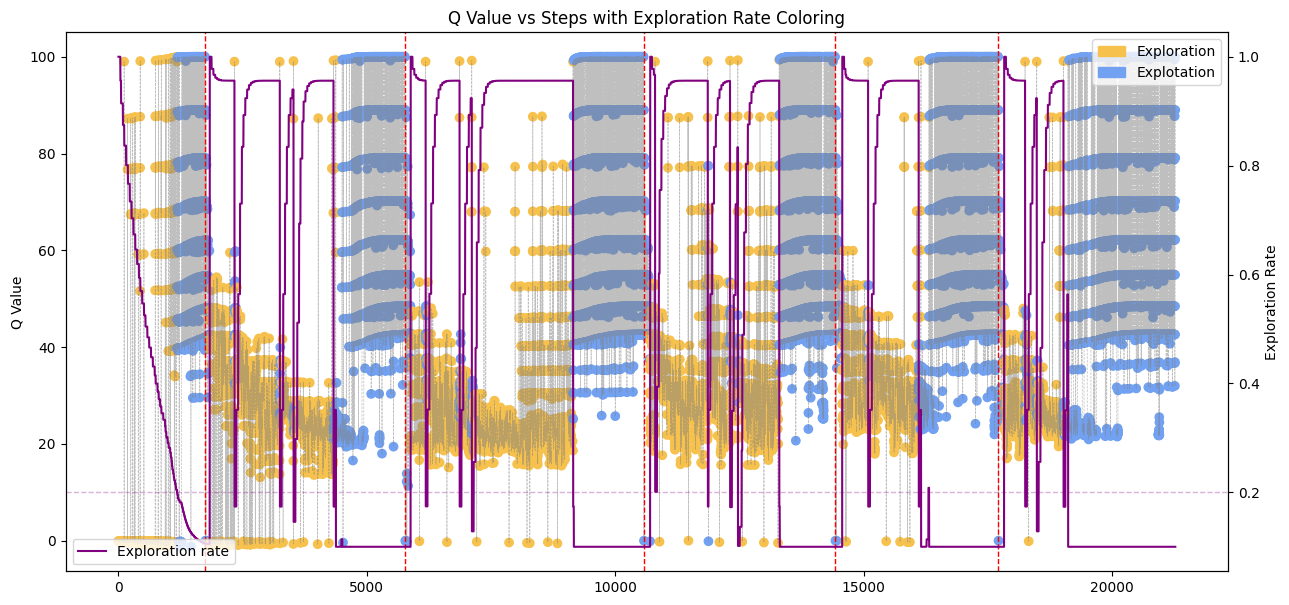
\includegraphics[width=\textwidth]{figures/epsilon.png}
    \caption{Figure description}
    \label{fig:epsilon}
\end{figure*}

These adaptive mechanisms equip the agent to effectively manage learning under varying and unpredictable conditions, enabling continuous adaptation and efficient knowledge transfer between different environmental states. This approach allows the agent to rapidly respond to new information without discarding previously learned knowledge, achieving greater resilience and performance stability over its lifespan. 

%%%%
\subsection{Agent adaptation to different goals}


%%%%
\subsection{Agent acquisition of new capabilities}


\endinput

